\documentclass[mat1]{fmfdelo}
% \documentclass[mat1, tisk]{fmfdelo}
% Če pobrišete možnost tisk, bodo povezave obarvane,
% na začetku pa ne bo praznih strani po naslovu, …

\avtor{Lenart Miklavič}
\naslov{Kompleksna eksponentna preslikava in kaos}
\title{The Complex Exponential Map and Chaos}
\mentor{doc.~dr.~Uroš Kuzman}
\letnica{2025}

% - povzetek v slovenščini
%   V povzetku na kratko opišite vsebinske rezultate dela. Sem ne sodi razlaga
%   organizacije dela, torej v katerem razdelku je kaj, pač pa le opis vsebine.
\povzetek{Dokažemo, da je kompleksna eksponentna preslikava \emph{kaotična}, ko
jo obravnavamo kot dinamični sistem na kompleksni ravnini. Pred tem je
obravnavana snov, ki je potrebna za razumevanje dokaza.}

% - Prevod slovenskega povzetka v angleščino.
\abstract{We prove that the complex exponential map is \emph{chaotic} when
considered as a dynamical system on the complex plane. The background necessary
for understanding the proof is covered beforehand.}

% - klasifikacijske oznake, ločene z vejicami
%   Oznake, ki opisujejo področje dela, so dostopne na strani https://www.ams.org/msc/
\klasifikacija{37F10, 30D05}

% - ključne besede, ki nastopajo v delu, ločene s \sep
\kljucnebesede{kaos\sep dinamični sistem\sep hiperbolična metrika}

% - angleški prevod ključnih besed
\keywords{chaos\sep dynamical system\sep hyperbolic metric}

% - angleško-slovenski slovar strokovnih izrazov
\slovar{
    \geslo{chaos}{kaos}
    \geslo{dynamical system}{dinamični sistem}
    \geslo{hyperbolic metric}{hiperbolična metrika}
    \geslo{density of hyperbolic metric}{gostota hiperbolične metrike}
}

\literatura{literatura.bib}
\usepackage[tracking=true,kerning=true,babel]{microtype}
\usepackage{mathtools}
\usepackage[exponent-product=\ensuremath{\cdot},output-decimal-marker={,}]{siunitx}
\usepackage{enumitem}
\usepackage{etoolbox}

\makeatletter
\usepackage{epigraph}
    \pretocmd{\@epitext}{\em}{}{}
    \apptocmd{\@epitext}{\em}{}{}
    \setlength{\epigraphrule}{0pt}
\makeatother

\newcommand{\NN}{\mathbb N}
\newcommand{\ZZ}{\mathbb Z}
\newcommand{\QQ}{\mathbb Q}
\newcommand{\RR}{\mathbb R}
\newcommand{\CC}{\mathbb C}
\newcommand{\DD}{\mathbb D}
\newcommand{\HH}{\mathbb H}

\newcommand{\TTT}{\mathcal T}
\newcommand{\OOO}{\mathcal O}
\newcommand{\DDD}{\mathcal D}

\newcommand{\dd}{\mathrm{d}}

\DeclareMathOperator{\Id}{Id}
\DeclareMathOperator{\re}{Re}
\DeclareMathOperator{\im}{Im}
\DeclareMathOperator{\Arg}{Arg}
\DeclareMathOperator{\diam}{diam}

\DeclarePairedDelimiter\absolute{\lvert}{\rvert}
\def\abs{\absolute*}
\DeclarePairedDelimiterXPP{\hderivative}[3]{}{\lVert}{\rVert}{_{#2}^{#3}}{\mathrm{D} #1}
\def\hder{\hderivative*}

\newcommand{\prt}[1]{\left( #1 \right)}
\newcommand{\set}[1]{\left\{ #1 \right\}}
\newcommand{\zap}[1]{\left\{ #1_n \right\}_{n = 1}^{\infty}}


\begin{document}

\section{Uvod} \label{sec:intro}

Naj bo \(x_0\) poljubno realno število. Opazujemo, kaj se dogaja z zaporedjem iteracij ali \emph{orbito} števila \(x_0\) glede na funkcijo \(e^{x}\):
\[x_0 \mapsto e^{x_0} \mapsto e^{e^{x_0}} \mapsto e^{e^{e^{x_0}}} \mapsto \cdots\]
Hitro se prepričamo, da je vsako tako zaporedje divergentno. Če pa zaporedje opazujemo kot iteracijo kompleksnega števila \(z_0\) glede na preslikavo \(e^z\):
\[z_0 \mapsto e^{z_0} \mapsto e^{e^{z_0}} \mapsto e^{e^{e^{z_0}}} \mapsto \cdots,\]
se stvar zaplete. Izkaže se, da na vsaki odprti množici obstajajo števila, katerih orbite se med seboj drastično razlikujejo.

\begin{izrek}[Orbite kompleksne eksponentne preslikave] \label{thm:orbits}
    Vsaka od naslednjih množic je za preslikavo \(f \colon \CC \to \CC\); \(z \mapsto e^{z}\) gosta v kompleksni ravnini:
    \begin{enumerate}
        \item množica števil, katerih orbita divergira k \(\infty\);
        \item množica števil, katerih orbita gosto pokrije kompleksno ravnino;
        \item množica periodičnih točk, to je števil \(z_0\), za katere obstaja \(k > 0\), da je \(z_k = z_0\).
    \end{enumerate}
\end{izrek}

\noindent Iz izreka nemudoma sledi, da je eksponentna preslikava \emph{kaotična}: pojem, ki ga bomo natančno definirali v razdelku \ref{sec:dis}. Za dokaz bomo potrebovali nekaj kompleksne analize ter rezultatov iz hiperbolične geometrije, ki so obravnavani v razdelku \ref{sec:hipgeom}. Preostanek dela je namenjen dokazu.

\section{Dinamični sistemi} \label{sec:dis}

V splošnem je dinamični sistem množica stanj skupaj z determinističnim evolucijskim pravilom. Množica stanj je običajno metrični ali topološki prostor \(X\), deterministično evolucijsko pravilo pa preslikava \(F \colon X \to X\). Dinamične sisteme delimo na

\begin{enumerate}
    \item \emph{diskretne} ali \emph{rekurzivne}, kjer je \(x_n \in X\) in
        \(x_{n + 1} = F (x_n)\);
    \item \emph{zvezne}, ki so sistemi diferencialnih enačb:
        \(\dot{\mathbf{x}} = F (\mathbf{x})\) za
        \(\mathbf{x} \in X \subseteq \RR^n\).
\end{enumerate}

\noindent V zgornjih primerih sta indeksni ali \emph{časovni} množici \(\NN\) in \(\RR\). Splošneje je to lahko poljuben monoid (glej \cite{Giunti_2012}).

\begin{zgled}
    Kompleksna števila \(\CC\) skupaj s kompleksno eksponentno preslikavo \(f \colon \CC \to \CC\); \(z \mapsto e^{z}\) so diskretni dinamični sistem.
\end{zgled}

\noindent Označimo \(f^n \coloneq f \circ f^{n - 1}\), kjer je
\(f^0 = \Id\).

\begin{definicija}
    Naj bo \(X\) množica in \(f \colon X \to X\) preslikava. \emph{Orbita} začetne točke \(x \in X\) pod preslikavo \(f\) je zaporedje \(a_n \coloneq f^n (x)\). Začetni točki pravimo
    \begin{itemize}
        \item \emph{ubežna}, če njena orbita divergira k \(\infty\);\footnote{To pomeni \(\lim_{n \to \infty} |f^n (z)| = \infty\).}
        \item \emph{periodična}, če obstaja tak \(n \in \NN\), da je \(f^n (x) = x\). Če je \(n\) najmanjše tako število, pravimo, da ima periodična točka periodo \(n\);
        \item \emph{fiksna}, če je periodična s periodo \(\num{1}\).
    \end{itemize}
\end{definicija}

\begin{definicija}[Topološka tranzitivnost]
    Naj bo \((X, \tau)\) topološki prostor in \(f \colon X \to X\) preslikava. Pravimo, da je \(f\) \emph{topološko tranzitivna}, če za vsaki \(U, V \in \tau\), obstajata \(z \in U\) in
    \(n \in \NN \cup \set{0}\), da je \(f^n (z) \in V\).
\end{definicija}

\begin{definicija}[Devaneyjev kaos]
    Naj bo \((M, d)\) metrični prostor in \(X \subseteq M\) neskončna. Pravimo, da je zvezna preslikava \(f \colon X \to X\) \emph{kaotična} (po Devaneyju), če sta izpolnjena naslednja pogoja.
    \begin{enumerate}
        \item Množica periodičnih točk je gosta v množici \(X\).
        \item Preslikava \(f\) je topološko tranzitivna.
    \end{enumerate}
\end{definicija}

\noindent Pojem kaosa je leta \num{1989} definiral ameriški matematik Robert L.~Devaney \cite{Devaney_1986}. Za kompleksno eksponentno preslikavo kot posledica sledi iz izreka 
\ref{thm:orbits}. Ta izrek je prvi dokazal poljski matematik Micha\l\ Misiurewicz leta \num{1981} \cite{Misiurewicz_1981}. S tem je potrdil domnevo, ki jo je leta \num{1926} postavil francoski matematik Pierre J.~L.~Fatou \cite{Fatou_1926}.
\section{Hiperbolična geometrija} \label{sec:hipgeom}

Hiperbolična geometrija se od evklidske razlikuje v tem, da aksiom

\begin{aksiom}
    Za poljubno premico \(p\) in točko \(A\), ki ne leži na premici \(p\), obstaja natanko ena premica \(q\), ki vsebuje \(A\) in ne seka premice \(p\).
\end{aksiom}

\noindent nadomestimo z

\begin{aksiom}
    Obstajata premica \(p\) in točka \(A\), ki ne leži na premici \(p\), tako, da obstajata vsaj dve premici \(q\) in \(r\), ki vsebujeta \(A\) in ne sekata premice \(p\).
\end{aksiom}

\noindent Nov aksiom prinaša veliko posledic, med drugim tudi drugo metriko; \emph{hiperbolično metriko}, katere lastnosti bomo uporabili pri dokazu. Metriko najprej definiramo na enotskem disku \(\DD \coloneq \set{z \in \CC : |z| < 1}\) in jo nato razširimo na bolj splošne množice. Za začetek ponovimo nekaj osnovnih pojmov iz kompleksne analize.

Uporabljamo standardne oznake. Kompleksno število \(z \in \CC\) lahko zapišemo kot vsoto \(z = x + i y\) ali v polarnem zapisu \(z = r e^{i \theta} = r (\cos \theta + i \sin \theta)\). Kot, ki ga oklepata abscisa in premica skozi \(0\) in \(z\), označimo z \(\Arg (z) \in (- \pi, \pi]\) ali \(\arg (z) \in [0, 2 \pi)\). Z \(\Delta (a, r)\) označimo odprt disk s središčem v \(a\) in radijem \(e\). Torej je \(\DD \coloneq \Delta (0, 1)\). Riemannovo sfero označimo z \(\hat{\CC} \coloneq \CC \cup \{\infty\}\).

% \begin{definicija}
%     Naj bo \(D\) odprta množica v \(\CC\) in \(f \colon D \to \CC\) funkcija. Če obstaja
%     \[f' (a) \coloneq \lim_{z \to a} \frac{f (z) - f (a)}{z - a},\]
%     tedaj število \(f' (a)\) imenujemo odvod funkcije \(f\) v točki \(a\). Če \(f' (a)\) obstaja za vsak \(a \in D\), potem pravimo, da je \(f\) \emph{holomorfna} funkcija na \(D\).
% \end{definicija}

\begin{definicija}
    Neprazni odprti in povezani podmnožici kompleksnih števil pravimo \emph{območje}.
\end{definicija}

\noindent Intuitivno si \emph{enostavno povezano} območje predstavljamo kot tisto območje, ki nima ``lukenj''. Natančno pa ga definiramo definiramo z naslednjim izrekom.

\begin{definicija}[Riemannov upodobitveni izrek]
    Območje \(D \subsetneq \CC\) je \emph{enostavno povezano} natanko tedaj, ko obstaja konformni izomorfizem (bijektivna holomorfna funkcija) \(\phi \colon D \to \DD\).
\end{definicija}

\vspace{0.5cm}
\noindent Pri dokazu izreka \ref{thm:orbits} si bomo pomagali tudi z inverzom eksponentne preslikave. Ker pa je \(e^{z + 2 \pi i} = e^x (\cos (y + 2 \pi) + i \sin (y + 2 \pi)) = e^z\), je eksponentna preslikava periodična (glej sliko \ref{fig:exponential}) in posledično nima inverza.
\begin{figure}
    \centering
    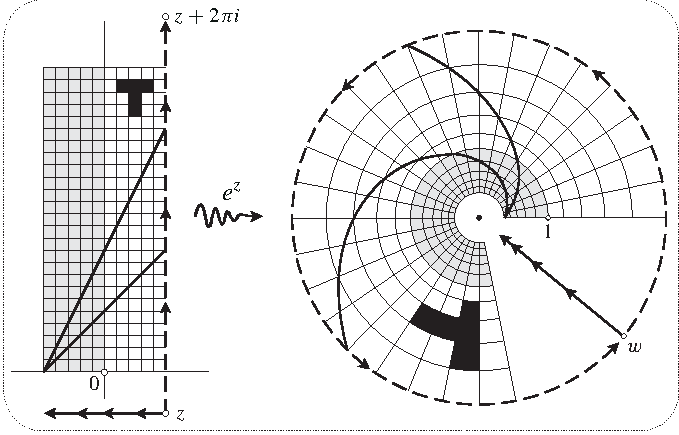
\includegraphics[width=0.6\textwidth]{needham_figure.pdf}
    \caption[Geometrijsko delovanje kompleksne eksponentne preslikave]{Geometrijska vizualizacija kompleksne eksponentne preslikave. Ilustracija je povzeta po knjigi \cite{Needham_1997}}
    \label{fig:exponential}
\end{figure}
Res, naj bo \(w = u + i v\). Rešimo enačbo:
\begin{align*}
    e^w = z &\iff e^u (\cos v + i \sin v) = x + i y\\
            &\iff e^u = \sqrt{x^2 + y^2} \quad \text{in} \quad v = \Arg z + 2 k \pi.
\end{align*}
Torej je \(e^w = z\) natanko tedaj, ko je
\[w = \ln |z| + i \Arg z + 2 k \pi i,\]
za vsak \(k \in \ZZ\). Prav tako bi lahko namesto \(\Arg\) izbrali \(\arg\). Da lahko definiramo inverz, moramo domeno omejiti. Naj bo \(\theta \in \RR\). Potem je
\[\begin{multlined}[10cm]
    \exp \colon  \set{\zeta \in \CC \colon \theta -\pi < \im \zeta < \theta + \pi}\\
    \to \set{\omega \in \CC \colon \Arg \omega \not\equiv \theta - \pi\ (\operatorname{mod}\, 2 \pi)} \eqcolon U
\end{multlined}\]
bijektivna na \(U\) in ima tam holomorfen inverz \(L \colon U \to \CC\):
\[L (\omega) \coloneq \log |\omega| + i \cdot \prt{\theta + \Arg \frac{\omega}{e^{i \theta}}}.\]
Vsaki taki funkciji \(L\) rečemo \emph{veja logaritma}. Če vzamemo \(\theta = 0\) dobimo \emph{glavno} vejo logaritma. Veje logaritma obstajajo tudi na vsakem preprosto povezanem območju, vendar bodo za nas pomembne le zarezane ravnine \(\CC \setminus [0, \infty)\) in diski, ki ne vsebuje izhodišča. Na primer, imejmo disk \(\Delta \subset \CC\), tako da \(0 \notin \Delta\). Naj bo \(\zeta_0 \in \CC\), da je \(e^{\zeta_0} \in \Delta\). Če vzamemo \(\theta = \im \zeta_0\), dobimo holomorfno preslikavo \(L \colon \Delta \to \CC\), za katero velja \(L (e^{\zeta_0}) = \zeta_0\) ter \(e^{L (\omega)} = \omega\) in \(\im \zeta_0 - \pi < \im L (\omega) < \im \zeta_0 + \pi\) za vsak \(\omega \in \Delta\).

\subsection{Hiperbolična metrika na enotskem disku}

Hiperbolično metriko podamo prek \emph{hiperboličnega ločnega elementa}:
\[\dd \rho_{\DD} (z) = \frac{2 |\dd z|}{1 - |z|^2},\]
ki nam pove, da se infinitezimalna sprememba v točki \(z\) v hiperbolični metriki izrazi kot infinitezimalna sprememba v evklidski metriki, pomnožena s t.i.~\emph{gostoto} hiperbolične metrike
\[\rho_{\DD} (z) = \frac{2}{1 - |z|^2}.\]
Iz tega izhaja naslednja definicija.

\begin{definicija}
    Naj bo \(\gamma \colon [a, b] \to \DD\) odsekoma \(C^1\) krivulja. Njena \emph{hiperbolična dolžina} je
    \[l_{\DD} (\gamma) \coloneq \int_{\gamma} \rho_{\DD} (z) \, | \dd z | = \int_{a}^{b} \frac{2 | \gamma' (t) | }{1 - | \gamma (t) |^2} \, \dd t.\]
\end{definicija}

\noindent Končno hiperbolično metriko definiramo kot sledi.

\begin{definicija}
    \emph{Hiperbolična metrika} je preslikava \(d_{\DD} \colon \DD \times \DD \to [0, \infty)\), definirana kot
    \[d_{\DD} (z, w) \coloneq \inf_{\gamma} l_{\DD} (\gamma),\]
    kjer \(\gamma\) teče po vseh odsekoma \(C^1\) krivuljah v \(\DD\), ki povezujejo točki \(z\) in \(w\).
\end{definicija}

\subsection{Hiperbolična metrika na enostavno povezanih območjih}

Definicijo nam iz enotskega diska na enostavno povezana območja prenese naslednji izrek.

\begin{izrek}[Pick] \label{thm:pick}
    Naj bosta \(U, V \subsetneq \CC\) enostavno povezani območji in \(f \colon U \to V\) holomorfna preslikava. Potem na \(U\) obstaja enolično določen hiperbolični ločni element, da velja naslednje.
    \begin{enumerate}
        \item Za vsak \(z \in \DD\) velja \(\rho_{\DD} (z) = \frac{2}{1 - |z|^2}\).
        \item Preslikava \(f\) ne veča \emph{hiperboličnega odvoda}, to je \[\hder{f (z)}{U}{V} \coloneq |f' (z)| \cdot \frac{\rho_V (f (z))}{\rho_U (z)} \leq 1.\]
        \item Enakost \(\hder{f (z)}{U}{V} = 1\) velja natanko tedaj, ko je \(f\) konformni izomorfizem.
        \item Če je \(U \subsetneq V\), potem za vsak \(z \in U\) velja \(\rho_U (z) > \rho_V (z)\). 
    \end{enumerate}
\end{izrek}

\noindent Druga in tretja točka sta pripravni za eksplicitno računanje gostot hiperbolične metrike.

\begin{trditev}[Zgledi hiperbolične metrike] \label{prop:hypexamples} \mbox{}
    \begin{enumerate}
        \item Za desno polravnino \(\HH \coloneq \set{ z \in \CC : \re (z) > 0 }\) je \(\rho_\HH = \frac{1}{\re (z)}\).
        \item Za zgornjo polravnino \(\KK \coloneq \set{z \in \CC : \im (z) > 0}\) je \(\rho_{\KK} (z) = \frac{1}{\im (z)}\)
        \item Za pas \(S \coloneq \set{z \in \CC : |\im (z)| < \pi}\) višine \(2 \pi\) je \(\rho_{S} = \frac{1}{2 \cos (\im (z) / 2)}\).
        \item Za zarezani ravnini velja
            \[
                \rho_{\CC \setminus [0, \infty)} (z) = \frac{1}{2 |z| \sin (\arg (z) / 2)},
                \qquad
                \rho_{\CC \setminus (-\infty, 0]} (z) = \frac{1}{2 |z| \cos (\Arg (z) / 2)}.
            \]
    \end{enumerate}
\end{trditev}

\begin{dokaz}
    Uporabimo izrek \ref{thm:pick} na štirih konformnih izomorfizmih. Naj bo \(\varphi_1 \colon \HH \to \DD\); \(z \mapsto (1 - z) / (1 + z)\). Potem je
    \[\rho_{\HH} (z) = \rho_{\DD} (\varphi_1 (z)) \cdot \abs{\varphi_1' (z)} = \frac{2}{1 - |\varphi_1 (z)|^2} \cdot \frac{2}{|z + 1|^2} = \frac{4}{|1 + z|^2 - |1- z|^2}.\]
    Za \(z = x + i y\) razpišemo \(|1 \pm z|^2 = 1 \pm 2x + x^2 + y^2\) in dobimo želen rezultat. Naj bo \(\varphi_2 (z) \colon \KK \to \DD\); \(\varphi_2 (z) = (z - i) / (z + i)\). Potem po zgornjem postopku dobimo
    \[\rho_{\KK} (z) = \rho_{\DD} (\varphi_2 (z)) \cdot \abs{\varphi_2' (z)} = \frac{4}{|z + i|^2 - |z - i|^2} = \frac{1}{\im (z)}.\]
    Naj bo \(\varphi_3 \colon S \to \HH\); \(z \mapsto e^{z / 2}\). Potem je
    \[\rho_S (z) = \rho_{\HH} (\varphi_2 (z)) \cdot |\varphi_2' (z)| = \frac{|\varphi_2 (z)|}{2 \re \varphi_2 (z)} = \frac{1}{2 \cos (\arg (\varphi_2 (z)))} = \frac{1}{2 \cos (\im (z) / 2)}.\]
    Naj bo \(\varphi_4 \colon \CC \setminus (- \infty, 0] \to \HH\); \(z \mapsto \sqrt{z}\). To je konformni izomorfizem, če se omejimo na rešitev \(r e^{i \theta} \mapsto \sqrt{r} e^{i \theta / 2}\) za \(\theta \in (- \pi, \pi)\). Potem je
    \[\rho_{\CC \setminus (- \infty, 0]} (z) = \rho_{\HH} (\varphi_4 (z)) \cdot |\varphi_4' (z)| = \frac{1}{2 |\sqrt{z}| \re (\sqrt{z})}.\]
    Dobljeno poenostavimo s polarnim zapisom, da dobimo
    \[\frac{1}{2 r \cos (\theta / 2)} = \frac{1}{2 |z| \cos (\Arg (z) / 2)}.\]
    % \[\rho_{\CC \setminus [0, \infty)} (z) = \rho_{\HH} (\varphi_2 (z)) \cdot |\varphi_2' (z)| = \frac{2 |z|}{\re (- z^2)}.\]
    % Uporabimo polarni zapis \(z = r e^{i \theta}\), da dobimo \(- z^2 = - r^2 e^{2 i \theta}\) in \(\re (- r^2 e^{2 i \theta}) = - r^2 \cos (2 \theta)\). Zato z uporabo formule \(\cos (2 \theta) = \cos^2 \theta - \sin^2 \theta\) dobimo
    % \[\frac{2 |z|}{\re (- z^2)} = \frac{2}{- r \cos (2 \theta)} = \frac{2}{r (\sin^2 \theta - \cos^2 \theta)}\]
\end{dokaz}

\section{Gostota ubežnih točk}

Od tu naprej naj velja, da \(f\) vedno označuje kompleksno eksponentno preslikavo
\[f \colon \CC \to \CC; \qquad z \mapsto e^{z}.\]

\begin{izrek} \label{thm:escapingdense}
    Ubežna množica kompleksne eksponentne preslikave
    \[I (f) \coloneq \set{z \in \CC : \lim_{n \to \infty} \abs{f^n (z)} = \infty}\]
    je gosta v kompleksni ravnini.
\end{izrek}

\noindent Pomagamo si z naslednjo lemo.

\begin{lema}[Eksponentna preslikava veča hiperbolično metriko] \label{lem:hyper}
    Kompleksna eksponentna preslikava lokalno širi hiperbolično metriko na \(U \coloneq \CC \setminus [0, \infty)\). To pomeni, da za vse \(\zeta \in f^{-1} (U)\) velja \(\hder{f (\zeta)}{U}{U} > 1\). Še več, naj bo \(\zap{\zeta}\) zaporedje v \(f^{-1} (U)\), za katero velja \[\lim_{n \to \infty} \hder{f (\zeta_n)}{U}{U} = 1.\] Potem velja
    \[\lim_{n \to \infty} \min \set{|\zeta_n|, \Arg (\zeta_n)} = 0.\]
\end{lema}

\begin{dokaz}
    Pišemo \(\zeta = r e^{i \theta}\), kjer je \(\theta \in (0, 2 \pi)\), in računamo po definiciji hiperboličnega odvoda ter uporabimo trditev \ref{prop:hypexamples}:
    \[
        \hder{f (\zeta)}{U}{U}
        =
        |f' (\zeta)| \cdot \frac{2 |\zeta| \cdot \sin \prt{\frac{1}{2} \arg (\zeta)}}{2 |e^{\zeta}| \cdot \sin \prt{\frac{1}{2} \arg (e^{\zeta})}}
        =
        \frac{r \cdot \sin (\theta / 2)}{\sin \prt{\frac{1}{2} \arg (e^{\zeta})}}.    
    \]
    Da poenostavimo imenovalec, opazimo, da je \(e^{\zeta} = e^{r (\cos \theta + i \sin \theta)}\) periodična s periodo \(2 \pi\). Zato velja \(\arg (e^{\zeta}) \equiv r \cdot \sin (\theta) \pmod{2 \pi}\). Dodatno je še \(|\sin|\) periodična s periodo \(\pi\) in zato \(|\sin (\arg (e^{\zeta}) / 2)| = |\sin (r \cdot \sin (\theta) / 2)|\). Zato velja
    \[\hder{f (\zeta)}{U}{U} = \frac{r \cdot \sin (\theta / 2)}{|\sin (\frac{r}{2} \cdot \sin (\theta))|}.\]
    Upoštevamo, da za vsak \(x \in \RR\) velja \(|\sin (x)| \leq |x|\):
    \[\hder{f (\zeta)}{U}{U} \geq \frac{r \cdot \sin (\theta / 2)}{\frac{r}{2} \cdot |\sin (\theta)|} = \frac{2 \cdot \sin (\theta / 2)}{|\sin (\theta)|}.\]
    Uporabimo formulo za dvojne kote \(\sin (2 x) = 2 \sin (x) \cos (x)\) in dobimo
    \begin{equation} \label{eqn:eta}
        \hder{f (\zeta)}{U}{U} \geq \frac{1}{|\cos (\theta / 2)|} > 1.
    \end{equation}

    \noindent Za drugi del dokaza pišemo \(\theta_n \coloneq \arg (\zeta_n)\). Po \eqref{eqn:eta} velja
    \[\hder{f (\zeta_n)}{U}{U} \geq \frac{1}{|\cos (\theta_n)|} > 1.\]
    Uporabimo predpostavke leme, iz česar sledi
    \[\lim_{n \to \infty} \frac{1}{|\cos (\theta_n)|} = 1\]
    in zato \(\lim_{n \to \infty} \Arg (\zeta_n)\).
\end{dokaz}

% \begin{lema}
%     Naj bo \(U\) kot prej in \(\zap{\theta}\) zaporedje v \(f^{-1 (U)}\). Tedaj je 
%     \[\lim_{n \to \infty} \hder{f (\zeta_n)}{U}{U} = 1\]
%     natanko tedaj, ko je
%     \[\lim_{n \to \infty} \Arg (\zeta_n) = 0 \qquad \text{in} \qquad \lim_{n \to \infty} \im \zeta_n = 0.\]
% \end{lema}

% \begin{dokaz}    
%     Pišemo \(\theta_n \coloneq \arg (\zeta_n)\) in predpostavimo, da \(\hder{f (\zeta_n)}{U}{U}\) konvergira proti \(\num{1}\). Po \eqref{eqn:eta} velja
%     \[\hder{f (\zeta_n)}{U}{U} \geq \frac{1}{|\cos (\theta_n)|} > 1.\]
%     Po predpostavki zato \[\lim_{n \to \infty} \frac{1}{|\cos (\theta_n)|} = 1\] in zato \(\lim_{n \to \infty} \Arg (\zeta_n) = 0\).
% \end{dokaz}

\begin{dokaz}[Dokaz izreka \ref{thm:escapingdense}]
    Naj bo \(w_0 \in \CC\) in \(w_n = f^n (w_0)\) za \(n \in \NN\). Naj bo \(D\) disk s središčem v \(w_0\). Vemo, da je \([0, \infty) \subset I (f)\), zato je dovolj, da dokažemo, da za nek \(n \in \NN\) velja \(f^n (D) \cap I (f) \neq \emptyset\). Dokazujemo s protislovjem, zato predpostavimo, da za vsak \(n \in \NN\) velja \(f^n (D) \cap I (f) = \emptyset\). Torej je
    \[D_n \coloneq f^n (D) \subset U = \CC \setminus [0, \infty) \qquad \text{za vsak } n \geq 0.\]
    Ker je \(f^n \colon D \to U\) holomorfna, velja Pickov izrek \ref{thm:pick} in zato
    \[\delta_n \coloneq \hder{f^n (w_0)}{D}{U} = |(f^n)' (w_0)| \cdot \frac{\rho_U (w_n)}{\rho_D (w_0)} \leq 1.\]
    Označimo \(\eta_n \coloneq \hder{f (w_n)}{U}{U}\) in opazimo \(\delta_{n + 1} = \delta_n \cdot \eta_n\) za vsak \(n \geq 0\). Po lemi \ref{lem:hyper} vemo, da je \(\eta_n > 1\). Zato je zaporedje \(\delta_n\) strogo naraščajoče in posledično konvergentno z limito \(\num{1}\). Lahko izračunamo
    \[\lim_{n \to \infty} \eta_n = \lim_{n \to \infty} \frac{\delta_{n + 1}}{\delta_n} = \frac{\lim_{n \to \infty} \delta_{n + 1}}{\lim_{n \to \infty} \delta_n} = 1.\]
    Spet po lemi \ref{lem:hyper} vemo
    \[\lim_{n \to \infty} \min \set{|w_n|, \Arg (w_n)} = 0.\]
    Zato morajo vsa stekališča zaporedja \(\zap{w}\) ležati na intervalu \([0, \infty)\). Ker \(w_0\) po predpostavki ni ubežna, množica stekališč ni prazna. Ker je tudi zaprta, ima minimum, ki ga označimo z \(z_0 \in [0, \infty)\). Po izreku obstaja podzaporedje \(w_{n_{k}}\), ki konvergira k \(z_0\). Opazimo, da velja
    \[\re w_{n_{k - 1}} = \log |w_{n_{k}}| \qquad \text{in} \qquad \lim_{k \to \infty} \log |w_{n_{k}}| = \log z_0 < z_0.\]
    Ker je \(z_0\) najmanjše stekališče zaporedja \(w_n\), podzaporedje \(w_{n_{k}}\) ne more imeti končnega stekališča in zato je
    \[\lim_{k \to \infty} |\im w_{n_{k-1}}| = \infty.\]
    To je v protislovju z \eqref{eqn:eta}.
\end{dokaz}

% Dokaz pušča odprto možnost, da ima množica ubežnih točk neprazno notranjost ali celo \(I (f) = \CC\). To izključimo z naslednjim izrekom.

% \begin{izrek}[Praslike negativnih realnih števil]
%     Naj bo \(W \subset \CC\) odprta in neprazna. Potem za neskončno mnogo \(n \geq 0\) velja \(f^{n} (W) \cap (- \infty, 0] \neq \emptyset\).
% \end{izrek}

% \begin{dokaz}
%     Naj bo \(D \subset W\) odprt disk. Najprej s protislovjem dokažemo, da obstaja vsaj en \(n\), da \(f^{n}\) seka \((- \infty, 0]\). Zato predpostavimo, da za vsak \(n \geq 0\) velja
%     \[f^{n} (D) \subset \tilde{U} \coloneq \CC \setminus (- \infty, 0].\]
%     Po izreku \ref{thm:escapingdense}, obstaja \(w_0 \in D \cap I (f)\).
% \end{dokaz}


\end{document}
